\chapter{Системы нечеткого вывода как метод анализа зашумленных или неопределенных входных данных}\label{ch:ch1}


Высокопроизводительный анализ данных (HPDM) позволяет обрабатывать и анализировать огромные массивы данных с использованием современных вычислительных технологий – как специализированных аппаратных средств (высокопроизводительных вычислительных кластеров, GPU ускорителей), так и оптимизированного программного обеспечения. Этот подход объединяет имеющиеся модели анализа данных с возможностями масштабируемых технологий Big Data и высокопроизводительных вычислений (HPC), что обеспечивает получение знаний на основе данных практически в реальном времени и значительно сокращает время от сбора данных до принятия обоснованных решений. Широкое промышленное применение получили программные пакеты (например, Apache Spark, NVIDIA RAPIDS), включающие традиционные модели анализа данных, а также инструменты JIT-компиляции готового программного кода (например, Numba).

Для определенных задач традиционные <<жёсткие>> вычисления (основанные на точных математических моделях) оказываются неэффективными или неприменимыми. Модели мягких вычислений принимают неопределённость, шум в данных и частичную истинность, что позволяет находить решения в условиях реального мира, где информация часто неполна или противоречива. Вместо строгих математических моделей используются эвристические и адаптивные методы, имитирующие человеческое мышление (например, лингвистические переменные вида <<высокая температура>>). Мягкие вычисления часто комбинируются с нейросетями (для обучения) и эволюционными алгоритмами (для оптимизации), усиливая их способность к обработке сложных систем.

Во многих случаях решение таких задач является вычислительно сложным, из-за чего технологии HPC оказываются востребованными в методах мягких вычислений. Наиболее ярко эта потребность выражается в задачах: планирование <<умных>> городов с использованием эволюционных алгоритмов для многокритериальной оптимизации \cite{Toutouh2019, Gora2015}, использование систем на основе нечеткой логике для управления и мониторинга производственных процессов в режиме реального времени \cite{Zhang2023, Vivas2022}, анализ сложных структур с большим количеством связей в задачах фармацевтики и генетики с применением генетических и роевых алгоритмов \cite{Liu2016, Easwaran2024}. Из этих примеров видно, что широкий спектр методов мягких вычислений хорошо поддаются распараллеливанию их алгоритмов.

Некоторые высокопроизводительные реализации нейро-нечетких систем были оформлены в самостоятельные программные модули. Частой практикой достижения высокой производительности нечетких систем является эффективная утилизация аппаратных ресурсов \cite{FuzzyLite}, в том числе, встраиваемых систем и плат ПЛИС \cite{Aldair2018}. В \cite{Lopez2015} и \cite{Elkano2017} представлена реализация схемы \textit{MapReduce} для классификации несбалансированных больших данных с использованием подхода Chi \cite{Chi1996}. В ситуации, когда большой набор данных целиком или фрагментарно может быть проанализирован с использованием памяти только одного вычислительного узла, но требуется провести много итераций анализа, для быстрого получения промежуточного результата нечеткого анализа целессообразно использовать (графический) ускоритель \cite{}.

% Мягкие вычисления (soft computing) --- это методология, объединяющая неточные и приближённые подходы для решения сложных задач, где традиционные «жёсткие» вычисления (основанные на точных математических моделях) оказываются неэффективными или неприменимыми. Понятие ввёл Лотфи Заде в 1994 году, и оно охватывает такие направления, как нечёткая логика, нейронные сети, эволюционные алгоритмы и вероятностные методы.

% Модели мягких вычислений принимают неопределённость, шум в данных и частичную истинность, что позволяет находить решения в условиях реального мира, где информация часто неполна или противоречива. Вместо строгих математических моделей используются эвристические и адаптивные методы, имитирующие человеческое мышление (например, лингвистические переменные вида «высокая температура»). Мягкие вычисления часто комбинируются с нейросетями (для обучения) и эволюционными алгоритмами (для оптимизации), усиливая их способность к обработке сложных систем.

% В отличие от жёстких вычислений, требующих точных моделей, мягкие вычисления фокусируются на адаптации к реальным условиям, где преобладает нечёткость. Например, они эффективны в анализе зашумлённых сигналов (как в ЭЭГ) или в системах управления, где решения принимаются на основе приближённых оценок. Также методы мягких вычислений используются для оценки параметров, где традиционные измерения затруднены (например, субъективные критерии качества).

% \todo{Ключевым элементом мягких вычислений являются нечёткие системы, которые преобразуют субъективные описания в структурированные решения через гранулирование информации — разбиение данных на семантические блоки. Это особенно важно в условиях неполных или противоречивых данных, где традиционные методы терпят неудачу. Таким образом, мягкие вычисления служат мостом между формальными моделями и реальным миром, предлагая гибкие и устойчивые к шумам решения.}

\section{Нейро-нечеткие системы}

Текущее развитие адаптивных нейро-нечетких систем (ANFIS) направлено на повышение применимости таких моделей за счет повышения точности моделирования и увеличения скорости получения результата моделирования. Прогресс по этим двум направлениям подкреплен экспериментами по использованию различных способов фаззификации \cite{Symmetry2021, Qian2023, Pekaslan2020}, импликации \cite{Shi2013, FernandezPeralta2025, Zhang2022, fern2021}, дефаззификации \cite{VanLeekwijck1999, Nasiboglu2022}, выборе $t$-норм, в том числе, $t$-норм в композиционном правиле вывода \cite{Pourabdollah2015}.

Например, в \cite{Wagner2016} предлагается использовать меру Жаккара между нечеткими множествами на входе и н. м. антецедента для определения уровня срабатывания правила в нейро-нечетких системах при несинглтонной фаззификации (NSFLS).

Существует также комбинированный подход с использованием так называемых гибких нейро-нечетких систем \cite{rutkovskiy2010, Cingolani2012}, сочетающих в себе два метода нечеткого вывода. Использование параметрических $t$-норм дает возможность осуществлять плавный переход от одного метода вывода к другому. Это позволяет совершать подбор оптимального метода вывода для конкретной задачи посредством оптимизации данного дополнительного гиперпараметра.

Чаще всего нейро-нечеткие системы используются для анализа четких входных данных взятых из четких наборов данных. Однако существуют примеры использования нечетких систем для моделирования нечетких данных. Например, прогнозирования временных рядов \cite{Pekaslan2020, Pourabdollah2017}.

Исследуются также и подходы для обучения нейро-нечетких систем. В работах широко применяется метод \cite{Wang1992} из-за своей простоты. Также появляются методы с использованием прогрессивных методов кластеризации правил \cite{Svetlakov2021}, эволюционного подхода \cite{}, градиентного спуска \cite{} и непрерывного обучения на потоковых данных \cite{Lima2010, Alves2021}.


\section{Методы нечеткого вывода}\label{sec:ch1-fuzzy-logical-inference-problem}

Эффективная организация нечеткого вывода является одной из главных точек повышения производительности при использовании нечетких систем. \todo{Проблема разрабатывается.} Предложенная в 1965 году Заде теория нечетких множеств \cite{zadeh1965} позже была использована для построения схемы нечеткого логического вывода \cite{Zadeh1996} и нечетких логических систем \cite{rutkovskiy2010}. Использование этой схемы нечеткого вывода для составных посылок оказывается затруднено из-за экспоненциальной временной сложности операций над нечеткими отношениями.

В ответ на проблему сложности использования классического нечеткого вывода спустя время появились методы Мамдани, Такаги-Сугено, Ларсена и Цукамото, вносящие в формулы нечеткого вывода упрощения для облегчения реализации. Упрощения прежде всего выражаются в использовании $t$-нормы вместо функции импликации, удовлетворяющей свойствам нечеткой импликации \cite{rutkovskiy2010}. Недостатком такого упрощения является искажение законов классической логики. Кроме того возникает расхождение при использовании лингвистической модели для анализа данных при многих правилах. Из-за этих недостатков данные подходы подвергаются критике.

В статьях \cite{Dubois2012, Izquierdo2018} авторы отмечают несколько наблюдений о различиях вывода типа Мамдани и логического типа при четких входах:
\begin{itemize}
	\item При полном соответствии входного нечеткого множестваа $A'$ одному из антецедентов $A' = A_i$ в подходе Мамдани нельзя получить на выходе $B' = B_i$ при срабатывании еще одного правила $A_j \ne A_i, j \ne i$, в отличии от конъюнкции правил при подходе Мамдани $B' = B_i \wedge B_j$.
	\item В подходе Мамдани при срабатывании в базе правил $R^M$ нескольких противоречивых правил выходное нечеткое множество всегда $A \circ R^M \ne \emptyset$, а выходное дефаззифицированное значений является усреднением центров противоречивых консеквентов $B_1$ и $B_2$. При этом точка $y$ может оказаться за пределами носителей нечетких множеств  $B_1$ и $B_2$, из-за чего для $\mu_{A'}(x_0)=1$ в полученной выходной точка $\mu_{B'}(y)=0$. В случае логического вывода такие правила взаимоисключаются, а на выходе будет получено пустое нечеткое множество $\emptyset$ при достаточном удалении друг от друга $B_1$ и $B_2$.
\end{itemize}

Изучение вопроса возможности использования несинглтонной фаззификации возродил и развил американский ученный Джерри Мендель \cite{Mendel2017}. Мендель привел аналитическое сравнение, показывающее, что NSFLS превосходят синглтонные нейро-нечетки системы в задаче прогнозирования зашумленных хаотических временных рядов благодаря своей способности учитывать неопределенность входных данных непосредственно при выводе. Он также сформировал доказательство того, что NSFLS является универсальным аппроксиматором любой непрерывной функции в некоторой области.

Однако исследования Менделя ограничены проработкой несинглтонной фаззификации в системах типа Мамдани и Такаги-Сугено, которые наследуют описанные выше расхождения с каноническим логическим выводом. Также формулы нечеткого вывода в его работах легко переписываются в удобный для вычисления вид, что достигается в упрощении в виде использования одной и той же $T$-нормы в выражении вывода, что сужает возможную вариативность нечеткой модели.

Таким образом на момент проведения исследования не существовало подходов обеспечивающих эффективный канонический нечеткий логический вывод Заде с возможностью полноценно обрабатывать фаззифицированные методом non-singleton входные значения. Актуальность решения описанной проблемы подтверждается:
\begin{enumerate}
	\item увеличением количества публикаций с использованием non-singleton фаззификации для вывода типа Мамдани за последние 10 лет, в которых достигается значимый прирост в качестве нечеткого моделирования;
	\item низкой проработанностью логического типа нечеткого вывода при non-singleton фаззификации, тогда как в определенных задачах синглтонный логический вывод превосходил по качеству моделирования метод Мамдани.
\end{enumerate}


%Предложенная в 1965 году Заде теория нечетких множеств \cite{zadeh1965} позже была использована для построения нечетких систем, которые нашли свое практическое применение в системах автоматизированного управления \cite{mamdani1975}, \cite{Lee1990}, прогнозирования временных последовательностей на зашумленных временных данных \cite{} и распознавания образов \cite{}.
%
%При нечетком выводе с использованием синглтонной фаззификации, входное значение рассматривается как точное значение измеряемой величины, исключающее какую-либо погрешность измерений. Несинглтонная фаззификация позволяет учесть эту погрешность и передать ее вместе с измеренным значением на вход нечеткого вывода. Такой тип систем был подробно изучен в \cite{mendel}.
%
%В отличии от синглтонной фаззификации, использование несинглтонной фаззификации в процедуре вывода имеет экспоненциальную вычислительную сложность при вычислении композиционного правила вывода. Некоторые работы пытаются направлены на обеспечение практической применимости нечетких систем на основе несинглтонной фаззификации \cite{liang}.
%
%Другая трудность в использовании несинглтонной фаззификации состоит в точном моделировании неопределенной во входных значениях. В большинстве случаев применения несинглтонной фаззификации предполагается, что неопределенность во входах одно из общеизвестных распределений, как правило, гауссовое [6] или треугольное. Для корректного определения характера шума во входных значениях может потребоваться проведение отдельного анализа. Также можно внедрить механизм адаптивного моделирования неопределенности в блок несинглтонной фаззификации нечеткой системы, который бы оценивал уровень шума на основе потока входных данных [2].

\section{Несинглтонная фаззификация}

Большинство имеющихся реализаций нечеткого вывода предоставляют возможность анализа лишь четких --- числовых данных.

\begin{figure}[ht]
	\centerfloat{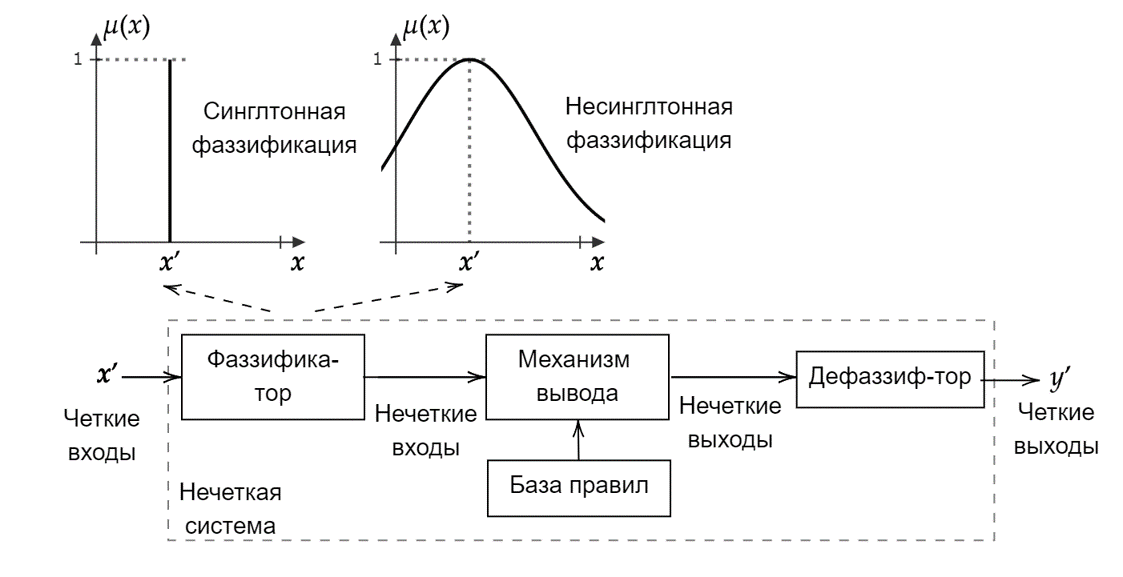
\includegraphics[scale=0.6]{singleton-vs-nonsingleton-fs}}
	\caption{Схема системы нечеткого вывода с использованием синглтонной и несинглтонной фаззификации}
	\label{fig:singleton-vs-nonsingleton}
\end{figure}

Нечеткая система представляется в виде композиции фаззификатора, базы правил, модуля вывода и дефаззификатора, как показано ра рисунке \cref{fig.signleton-vs-nonsingleton}. Фаззификация --- отображение входных данных из исходного пространства в пространство нечетких множеств. Наиболее распространенным является метод синглтонной фаззфикации. Основная причина его широкого использования является существенное упрощение реализации систем нечеткого вывода. При использовании синглтонной фаззификации поданное на вход значение $x'$ интерпретируется как истинное значение измеренной величины, что эквивалентно использованию функции принадлежности входного нечеткого множества $\mu_{A'}(x) = \left[x = x'\right]$. Информация о неопределенности входных данных при этом игнорируется.

Альтернативный подход с использованием несинглтонной фаззификации предусматривает формализацию входного значения нечетким множеством, содержащим информацию о неопределенности значения точки входных данных. Эти неопределенности могут возникать как результат несовершенства процедуры измерений (например, шумом измерительного оборудования, дефектами или деградацией качества датчиков), или когда входные данные описываются качественными понятиями естественного языка.

В случае с анализом числовых данных, неопределенность измерений формализуется функцией принадлежности, которая $\mu_{A'}(x') = 1$ и $\mu_{A'}(x)$ уменьшается по мере удаления от $x'$. При таком способе моделирования измеренное значение $x'$ рассматривается как истинное, а значения в его окрестности --- как возможные.

\begin{figure}[ht]
	\begin{minipage}[b][][b]{0.3\linewidth}
		\centering
		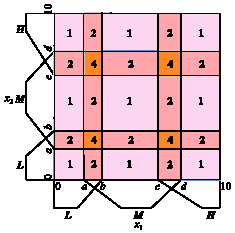
\includegraphics[width=\linewidth, page=1]{ns-fuz-mendel-comparizon-first-order-partition} \\ а) $\sigma_{A'} = 0\%$
	\end{minipage}
	\hfill
	\begin{minipage}[b][][b]{0.3\linewidth}
		\centering
		\includegraphics[width=\linewidth, page=2]{ns-fuz-mendel-comparizon-first-order-partition} \\ б) $\sigma_{A'} = 4\%$
	\end{minipage}
	\hfill
	\begin{minipage}[b][][b]{0.3\linewidth}
		\centering
		\includegraphics[width=\linewidth, page=3]{ns-fuz-mendel-comparizon-first-order-partition} \\ в)  $\sigma_{A'} = 12\%$
	\end{minipage}

    \caption{Сравнение областей активации правил при переходе от синглтонной фаззификации к несинглтонной и при увеличении ширины окрестности погрешности $\sigma_{A'}$.}
\end{figure}

Влияние перехода от синглтонной фаззификации к несинглтонной и величины окрестности погрешности на внутренее поведение и итоговое качество нечеткой системы продемонстрировал Мендель в \cite{Mendel2021, Mendel2017}. 

Для анализа влияния от использования того или иного способа фаззификации на корректность получаемого результата в статье \cite{Mendel2020} рассматривается карта разбиений первого и второго порядка на декартовом произведении базовых множеств входных лингвистических переменных. Мендель в своей книге проводил такое сравнение для систем типа Мамдани. Поскольку в системах типа Мамдани в качестве функции импликации выступает $t$-норма, то разница от применения двух способов фаззификации проявляется в различных максимальных уровнях линии пересечения ф. п. входной посылки и антецедента правила. %В зависимости от минимум или произведение. 

Применение композиционного правила вывода $\sup$ здесь дает эффект \textit{префильтрации} (или \textit{корректировки}) входного значения. То есть ядра функций принадлежности антецедентов правил выполняют функцию эталонов, а уровень пересечения функции принадлежности для входного значения и ф. п. антецедента правила позволяет интерпретировать входное значение как суперпозицию эталонных значений антецедентов с долями равными этому уровню.

 %Разбиение первого порядка 

\pgfmathdeclarefunction{gauss}{3}{%
  \pgfmathparse{exp(-((#1-#2)/(2*#3))^2)} % Correct syntax for Gaussian function
}
\pgfmathdeclarefunction{implL}{4}{%
  \pgfmathparse{min(1, 1-#4+gauss(#1, #2, #3))} % Lukasievich
}
\pgfmathdeclarefunction{implR}{4}{%
  \pgfmathparse{min(1, gauss(#1, #2, #3)/#4)} % R
}

\pgfplotsset{
    membership axes/.style={
        width=0.20\textwidth,
        height=0.20\textwidth,
        scale only axis,
        domain=0:1,
        samples=100,
        every axis plot/.append style={smooth},
        axis lines=middle,
        xmin=0, xmax=1,
        ymin=0, ymax=1,
        xticklabel style={font=\tiny, inner sep=1pt, outer sep=0pt},
        yticklabel style={font=\tiny, inner sep=1pt, outer sep=0pt},
    }
}

\begin{figure}[ht]
    \centering
    \begin{subfigure}[b]{\textwidth}
        \begin{tikzpicture}

        %\begin{scope}[xshift=0cm, yshift=0cm]
            \pgfmathsetmacro{\aZeroMu}{0.55}
            \pgfmathsetmacro{\aFstMu}{0.28}
            \pgfmathsetmacro{\aFstSigma}{0.09}
            \pgfmathsetmacro{\aFstCrossX}{0.55}
            \pgfmathsetmacro{\aFstCrossY}{0.11}
            \pgfmathsetmacro{\aSndMu}{0.5}
            \pgfmathsetmacro{\aSndSigma}{0.08}
            \pgfmathsetmacro{\aSndCrossX}{0.55}
            \pgfmathsetmacro{\aSndCrossY}{0.91}
            \pgfmathsetmacro{\aTrdMu}{0.89}
            \pgfmathsetmacro{\aTrdSigma}{0.2}
            \pgfmathsetmacro{\aTrdCrossX}{0.55}
            \pgfmathsetmacro{\aTrdCrossY}{0.49}
            \pgfmathsetmacro{\bFstMu}{0.2}
            \pgfmathsetmacro{\bFstSigma}{0.12}
            \pgfmathsetmacro{\bSndMu}{0.5}
            \pgfmathsetmacro{\bSndSigma}{0.1}
            \pgfmathsetmacro{\bTrdMu}{0.8}
            \pgfmathsetmacro{\bTrdSigma}{0.1}

            % First function
            \begin{axis}[
                membership axes,
                name=plot1,
                at={(0,0)},
                xlabel={$x_1$},
                ylabel={$\mu$},
                xlabel style={font=\footnotesize, at=(current axis.south), anchor=north, yshift=-10pt},
                ylabel style={font=\footnotesize, at=(current axis.west), anchor=east, xshift=-10pt},
            ]
                \addplot[blue, name path=A0] coordinates {(\aZeroMu, 0) (\aZeroMu, 1)};
                \addplot[black, name path=A1] {gauss(\x, \aFstMu, \aFstSigma)};
                \addplot[only marks, mark=*, mark size=2pt, purple!50] coordinates {(\aFstCrossX,\aFstCrossY)};
                \coordinate (fire11) at (axis cs:\aFstCrossX,\aFstCrossY); % USE axis cs
            \end{axis}
            % Second function
            \begin{axis}[
                membership axes,
                name=plot2,
                at={(0.25\textwidth,0)},
                xlabel={$x_2$},
                ylabel={$\mu$},
                xlabel style={font=\footnotesize, at=(current axis.south), anchor=north, yshift=-10pt},
                ylabel style={font=\footnotesize, at=(current axis.west), anchor=east, xshift=-10pt},
            ]
                \addplot[blue, name path=A0] coordinates {(\aZeroMu, 0) (\aZeroMu, 1)};
                \addplot[black, name path=A1] {gauss(\x, \aSndMu, \aSndSigma)};
                \addplot[only marks, mark=*, mark size=2pt, lime] coordinates {(\aSndCrossX,\aSndCrossY)};
                \coordinate (fire12) at (axis cs:\aSndCrossX,\aSndCrossY); % Use axis cs
            \end{axis}
            % Third function
            \begin{axis}[
                membership axes,
                name=plot3,
                at={(0.5\textwidth,0)},
                xlabel={$x_3$},
                ylabel={$\mu$},
                xlabel style={font=\footnotesize, at=(current axis.south), anchor=north, yshift=-10pt},
                ylabel style={font=\footnotesize, at=(current axis.west), anchor=east, xshift=-10pt},
            ]
                \addplot[blue, name path=A0] coordinates {(\aZeroMu, 0) (\aZeroMu, 1)};
                \addplot[black, name path=A1] {gauss(\x, \aTrdMu, \aTrdSigma)};
                \addplot[only marks, mark=*, mark size=2pt, cyan!50] coordinates {(\aTrdCrossX,\aTrdCrossY)};
                \coordinate (fire13) at (axis cs:\aTrdCrossX,\aTrdCrossY); % Use axis cs
            \end{axis}
            % Fourth function
            \begin{axis}[
                membership axes,
                name=plot4,
                at={(0.75\textwidth,0)},
                xlabel={$y$},
                ylabel={$\mu_{B'}(y)$},
                xlabel style={font=\footnotesize, at=(current axis.south), anchor=north, yshift=-10pt},
                ylabel style={font=\footnotesize, at=(current axis.above origin), anchor=south},
            ]
                \addplot [purple!50] {min(\aFstCrossY, gauss(\x, \bFstMu, \bFstSigma))};
                \addplot [lime] {min(\aSndCrossY, gauss(\x, \bSndMu, \bSndSigma))};
                \addplot [cyan!50] {min(\aTrdCrossY, gauss(\x, \bTrdMu, \bTrdSigma))};
                \addplot[fill=orange!30, orange] {max(min(\aFstCrossY, gauss(\x, \bFstMu, \bFstSigma)), min(\aSndCrossY, gauss(\x, \bSndMu, \bSndSigma)), min(\aTrdCrossY, gauss(\x, \bTrdMu, \bTrdSigma)))} \closedcycle;
                \coordinate (out11) at (axis cs:0.0,\aFstCrossY); % Use axis cs
                \coordinate (out12) at (axis cs:0.0,\aSndCrossY); % Use axis cs
                \coordinate (out13) at (axis cs:0.0,\aTrdCrossY); % Use axis cs
            \end{axis}

            % Connect coordinates using defined coordinate names
            \draw [purple!50, dashed, thick] (fire11) -- (out11);
            \draw [lime, dashed, thick] (fire12) -- (out12);
            \draw [cyan!50, dashed, thick] (fire13) -- (out13);

            % \node {\sigma=\aZeroSigma};
            \node[left, xshift=-1.2cm, font=\footnotesize, rotate=90, anchor=center] at (plot1.west) {$\sigma_{A'}=0$};
        \end{tikzpicture}
	\end{subfigure}
	
	%%
	\vspace{0.1cm}
	%%
	
	\begin{subfigure}[b]{\textwidth}
        \begin{tikzpicture}

        %\begin{scope}[xshift=0cm, yshift=0cm]
            \pgfmathsetmacro{\aZeroMu}{0.55}
            \pgfmathsetmacro{\aZeroSigma}{0.01}
            \pgfmathsetmacro{\aFstMu}{0.28}
            \pgfmathsetmacro{\aFstSigma}{0.09}
            \pgfmathsetmacro{\aFstCrossX}{0.515}
            \pgfmathsetmacro{\aFstCrossY}{0.185}
            \pgfmathsetmacro{\aSndMu}{0.5}
            \pgfmathsetmacro{\aSndSigma}{0.08}
            \pgfmathsetmacro{\aSndCrossX}{0.56}
            \pgfmathsetmacro{\aSndCrossY}{0.88}
            \pgfmathsetmacro{\aTrdMu}{0.89}
            \pgfmathsetmacro{\aTrdSigma}{0.2}
            \pgfmathsetmacro{\aTrdCrossX}{0.57}
            \pgfmathsetmacro{\aTrdCrossY}{0.53}
            \pgfmathsetmacro{\bFstMu}{0.2}
            \pgfmathsetmacro{\bFstSigma}{0.12}
            \pgfmathsetmacro{\bSndMu}{0.5}
            \pgfmathsetmacro{\bSndSigma}{0.1}
            \pgfmathsetmacro{\bTrdMu}{0.8}
            \pgfmathsetmacro{\bTrdSigma}{0.1}

            % First function
            \begin{axis}[
                membership axes,
                name=plot1,
                at={(0,0)},
                xlabel={$x_1$},
                ylabel={$\mu$},
                xlabel style={},
                xlabel style={font=\footnotesize, at=(current axis.south), anchor=north, yshift=-10pt},
                ylabel style={font=\footnotesize, at=(current axis.west), anchor=east, xshift=-10pt},
            ]
                \addplot[blue, name path=A0] {gauss(\x, \aZeroMu, \aZeroSigma)};
                \addplot[black, name path=A1] {gauss(\x, \aFstMu, \aFstSigma)};
                \addplot[fill=purple!50, draw=none] {min(gauss(\x, \aZeroMu, \aZeroSigma), gauss(\x, \aFstMu, \aFstSigma))} \closedcycle;
                \coordinate (fire11) at (axis cs:\aFstCrossX,\aFstCrossY); % USE axis cs
            \end{axis}
            % Second function
            \begin{axis}[
                membership axes,
                name=plot2,
                at={(0.25\textwidth,0)},
                xlabel={$x_2$},
                ylabel={$\mu$},
                xlabel style={font=\footnotesize, at=(current axis.south), anchor=north, yshift=-10pt},
                ylabel style={font=\footnotesize, at=(current axis.west), anchor=east, xshift=-10pt},
            ]
                \addplot[blue, name path=A0] {gauss(\x, \aZeroMu, \aZeroSigma)};
                \addplot[black, name path=A1] {gauss(\x, \aSndMu, \aSndSigma)};
                \addplot[fill=lime, draw=none] {min(gauss(\x, \aZeroMu, \aZeroSigma), gauss(\x, \aSndMu, \aSndSigma))} \closedcycle;
                \coordinate (fire12) at (axis cs:\aSndCrossX,\aSndCrossY); % Use axis cs
            \end{axis}
            % Third function
            \begin{axis}[
                membership axes,
                name=plot3,
                at={(0.5\textwidth,0)},
                xlabel={$x_3$},
                ylabel={$\mu$},
                xlabel style={font=\footnotesize, at=(current axis.south), anchor=north, yshift=-10pt},
                ylabel style={font=\footnotesize, at=(current axis.west), anchor=east, xshift=-10pt},
            ]
                \addplot[blue, name path=A0] {gauss(\x, \aZeroMu, \aZeroSigma)};
                \addplot[black, name path=A1] {gauss(\x, \aTrdMu, \aTrdSigma)};
                \addplot[fill=cyan!50, draw=none] {min(gauss(\x, \aZeroMu, \aZeroSigma), gauss(\x, \aTrdMu, \aTrdSigma))} \closedcycle;
                \coordinate (fire13) at (axis cs:\aTrdCrossX,\aTrdCrossY); % Use axis cs
            \end{axis}
            % Fourth function
            \begin{axis}[
                membership axes,
                name=plot4,
                at={(0.75\textwidth,0)},
                xlabel={$y$},
                ylabel={$\mu_{B'}(y)$},
                xlabel style={font=\footnotesize, at=(current axis.south), anchor=north, yshift=-10pt},
                ylabel style={font=\footnotesize, at=(current axis.above origin), anchor=south},
            ]
                \addplot [purple!50] {min(\aFstCrossY, gauss(\x, \bFstMu, \bFstSigma))};
                \addplot [lime] {min(\aSndCrossY, gauss(\x, \bSndMu, \bSndSigma))};
                \addplot [cyan!50] {min(\aTrdCrossY, gauss(\x, \bTrdMu, \bTrdSigma))};
                \addplot[fill=orange!30, orange] {max(min(\aFstCrossY, gauss(\x, \bFstMu, \bFstSigma)), min(\aSndCrossY, gauss(\x, \bSndMu, \bSndSigma)), min(\aTrdCrossY, gauss(\x, \bTrdMu, \bTrdSigma)))} \closedcycle;
                \coordinate (out11) at (axis cs:0.0,\aFstCrossY); % Use axis cs
                \coordinate (out12) at (axis cs:0.0,\aSndCrossY); % Use axis cs
                \coordinate (out13) at (axis cs:0.0,\aTrdCrossY); % Use axis cs
            \end{axis}

            % Connect coordinates using defined coordinate names
            \draw [purple!50, dashed, thick] (fire11) -- (out11);
            \draw [lime, dashed, thick] (fire12) -- (out12);
            \draw [cyan!50, dashed, thick] (fire13) -- (out13);

            % \node {\sigma=\aZeroSigma};
            \node[left, xshift=-1.2cm, font=\footnotesize, rotate=90, anchor=center] at (plot1.west) {$\sigma_{A'}=\aZeroSigma$};
        \end{tikzpicture}
	\end{subfigure}
	
	%%
	\vspace{0.1cm}
	%%
	
	\begin{subfigure}[b]{\textwidth}
          \begin{tikzpicture}
            \pgfmathsetmacro{\aZeroMu}{0.55}
            \pgfmathsetmacro{\aZeroSigma}{0.05}
            \pgfmathsetmacro{\aFstMu}{0.28}
            \pgfmathsetmacro{\aFstSigma}{0.09}
            \pgfmathsetmacro{\aFstCrossX}{0.49}
            \pgfmathsetmacro{\aFstCrossY}{0.4}
            \pgfmathsetmacro{\aSndMu}{0.5}
            \pgfmathsetmacro{\aSndSigma}{0.08}
            \pgfmathsetmacro{\aSndCrossX}{0.53}
            \pgfmathsetmacro{\aSndCrossY}{0.97}
            \pgfmathsetmacro{\aTrdMu}{0.89}
            \pgfmathsetmacro{\aTrdSigma}{0.2}
            \pgfmathsetmacro{\aTrdCrossX}{0.6}
            \pgfmathsetmacro{\aTrdCrossY}{0.61}
            \pgfmathsetmacro{\bFstMu}{0.2}
            \pgfmathsetmacro{\bFstSigma}{0.12}
            \pgfmathsetmacro{\bSndMu}{0.5}
            \pgfmathsetmacro{\bSndSigma}{0.1}
            \pgfmathsetmacro{\bTrdMu}{0.8}
            \pgfmathsetmacro{\bTrdSigma}{0.1}

            % First function
            \begin{axis}[
                membership axes,
                name=plot1,
                at={(0,0)},
                xlabel={$x_1$},
                ylabel={$\mu$},
                xlabel style={font=\footnotesize, at=(current axis.south), anchor=north, yshift=-10pt},
                ylabel style={font=\footnotesize, at=(current axis.west), anchor=east, xshift=-10pt},
            ]
                \addplot[blue, name path=A0] {gauss(\x, \aZeroMu, \aZeroSigma)};
                \addplot[black, name path=A1] {gauss(\x, \aFstMu, \aFstSigma)};
                \addplot[fill=purple!50, draw=none] {min(gauss(\x, \aZeroMu, \aZeroSigma), gauss(\x, \aFstMu, \aFstSigma))} \closedcycle;
                \coordinate (fire11) at (axis cs:\aFstCrossX,\aFstCrossY); % USE axis cs
            \end{axis}
            % Second function
            \begin{axis}[
                membership axes,
                name=plot2,
                at={(0.25\textwidth,0)},
                xlabel={$x_2$},
                ylabel={$\mu$},
                xlabel style={font=\footnotesize, at=(current axis.south), anchor=north, yshift=-10pt},
                ylabel style={font=\footnotesize, at=(current axis.west), anchor=east, xshift=-10pt},
            ]
                \addplot[blue, name path=A0] {gauss(\x, \aZeroMu, \aZeroSigma)};
                \addplot[black, name path=A1] {gauss(\x, \aSndMu, \aSndSigma)};
                \addplot[fill=lime, draw=none] {min(gauss(\x, \aZeroMu, \aZeroSigma), gauss(\x, \aSndMu, \aSndSigma))} \closedcycle;
                \coordinate (fire12) at (axis cs:\aSndCrossX,\aSndCrossY); % Use axis cs
            \end{axis}
            % Third function
            \begin{axis}[
                membership axes,
                name=plot2,
                at={(0.5\textwidth,0)},
                xlabel={$x_3$},
                ylabel={$\mu$},
                xlabel style={font=\footnotesize, at=(current axis.south), anchor=north, yshift=-10pt},
                ylabel style={font=\footnotesize, at=(current axis.west), anchor=east, xshift=-10pt},
            ]
                \addplot[blue, name path=A0] {gauss(\x, \aZeroMu, \aZeroSigma)};
                \addplot[black, name path=A1] {gauss(\x, \aTrdMu, \aTrdSigma)};
                \addplot[fill=cyan!50, draw=none] {min(gauss(\x, \aZeroMu, \aZeroSigma), gauss(\x, \aTrdMu, \aTrdSigma))} \closedcycle;
                \coordinate (fire13) at (axis cs:\aTrdCrossX,\aTrdCrossY); % Use axis cs
            \end{axis}
            % Fourth function
            \begin{axis}[
                membership axes,
                name=plot4,
                at={(0.75\textwidth,0)},
                xlabel={$y$},
                ylabel={$\mu_{B'}(y)$},
                xlabel style={font=\footnotesize, at=(current axis.south), anchor=north, yshift=-10pt},
                ylabel style={font=\footnotesize, at=(current axis.above origin), anchor=south},
            ]
                \addplot [purple!50] {min(\aFstCrossY, gauss(\x, \bFstMu, \bFstSigma))};
                \addplot [lime] {min(\aSndCrossY, gauss(\x, \bSndMu, \bSndSigma))};
                \addplot [cyan!50] {min(\aTrdCrossY, gauss(\x, \bTrdMu, \bTrdSigma))};
                \addplot[fill=orange!30, orange] {max(min(\aFstCrossY, gauss(\x, \bFstMu, \bFstSigma)), min(\aSndCrossY, gauss(\x, \bSndMu, \bSndSigma)), min(\aTrdCrossY, gauss(\x, \bTrdMu, \bTrdSigma)))} \closedcycle;
                \coordinate (out11) at (axis cs:0.0,\aFstCrossY); % Use axis cs
                \coordinate (out12) at (axis cs:0.0,\aSndCrossY); % Use axis cs
                \coordinate (out13) at (axis cs:0.0,\aTrdCrossY); % Use axis cs
            \end{axis}

            % Connect coordinates using defined coordinate names
            \draw [purple!50, dashed, thick] (fire11) -- (out11);
            \draw [lime, dashed, thick] (fire12) -- (out12);
            \draw [cyan!50, dashed, thick] (fire13) -- (out13);

            % \node {\sigma=\aZeroSigma};
            \node[left, xshift=-1.2cm, font=\footnotesize, rotate=90, anchor=center] at (plot1.west) {$\sigma_{A'}=\aZeroSigma$};
        \end{tikzpicture}
    \end{subfigure}
    \caption{Сравнение формы функций принадлежности выходных нечетких множеств для подхода Мамдани}
    \label{fig:ns-width-influence-to-out-mamdani}
\end{figure}

Показанная на этих схемах динамика более ясно раскрыта на рисунке \cref{fig:ns-width-influence-to-out-mamdani} для различных значениях среднеквадратичного отклонения в гауссовой ф. п. входного значения на примере агрегации выходной ф. п. нечеткой системы с тремя правилами в базе правил. Видно, что при переходе от синглтонной фаззификации к несинглтонной и при дальнейшем увеличении ширины среднеквадратичного отклонения ф. п. входного нечеткого множества, повышается уровень срабатывания первого правила, и, как следствие использования импликации Мамдани, уровень задействования ф. п. выходного нечеткого множества этого правила в результирующей агрегации. Кроме того, можно пронаблюдать, упомянутый ранее, эффект корректировки входного значения антецедентом третьего правила.

В случае с нечеткой системой логического типа, разница от использования различных способов фаззификации будет проявляться в различных формах выходного нечеткого множества. 

\begin{figure}[ht]
    \centering
    \begin{subfigure}[b]{\textwidth}
        \begin{tikzpicture}

        %\begin{scope}[xshift=0cm, yshift=0cm]
            \pgfmathsetmacro{\aZeroMu}{0.55}
            \pgfmathsetmacro{\aFstMu}{0.28}
            \pgfmathsetmacro{\aFstSigma}{0.09}
            \pgfmathsetmacro{\aFstCrossX}{0.55}
            \pgfmathsetmacro{\aFstCrossY}{0.11}
            \pgfmathsetmacro{\aSndMu}{0.5}
            \pgfmathsetmacro{\aSndSigma}{0.08}
            \pgfmathsetmacro{\aSndCrossX}{0.55}
            \pgfmathsetmacro{\aSndCrossY}{0.91}
            \pgfmathsetmacro{\aTrdMu}{0.89}
            \pgfmathsetmacro{\aTrdSigma}{0.2}
            \pgfmathsetmacro{\aTrdCrossX}{0.55}
            \pgfmathsetmacro{\aTrdCrossY}{0.49}
            \pgfmathsetmacro{\bFstMu}{0.2}
            \pgfmathsetmacro{\bFstSigma}{0.12}
            \pgfmathsetmacro{\bSndMu}{0.5}
            \pgfmathsetmacro{\bSndSigma}{0.1}
            \pgfmathsetmacro{\bTrdMu}{0.8}
            \pgfmathsetmacro{\bTrdSigma}{0.1}

            % First function
            \begin{axis}[
                membership axes,
                name=plot1,
                at={(0,0)},
                xlabel={$x_1$},
                ylabel={$\mu$},
                xlabel style={font=\footnotesize, at=(current axis.south), anchor=north},
                ylabel style={font=\footnotesize, at=(current axis.west), anchor=east, xshift=-10pt},
                y dir=reverse,
                % axis x line=top,
                xticklabel pos=upper,
                xticklabel style={yshift=13pt}
            ]
                \addplot[blue, name path=A0] coordinates {(\aZeroMu, 0) (\aZeroMu, 1)};
                \addplot[black, name path=A1] {gauss(\x, \aFstMu, \aFstSigma)};
                \addplot[only marks, mark=*, mark size=2pt, purple!50] coordinates {(\aFstCrossX,\aFstCrossY)};
                \coordinate (fire11) at (axis cs:\aFstCrossX,\aFstCrossY); % USE axis cs
            \end{axis}
            % Second function
            \begin{axis}[
                membership axes,
                name=plot2,
                at={(0.25\textwidth,0)},
                xlabel={$x_2$},
                ylabel={$\mu$},
                xlabel style={font=\footnotesize, at=(current axis.south), anchor=north},
                ylabel style={font=\footnotesize, at=(current axis.west), anchor=east, xshift=-10pt},
                y dir=reverse,
                % axis x line=top,
                xticklabel pos=upper,
                xticklabel style={yshift=13pt}
            ]
                \addplot[blue, name path=A0] coordinates {(\aZeroMu, 0) (\aZeroMu, 1)};
                \addplot[black, name path=A1] {gauss(\x, \aSndMu, \aSndSigma)};
                \addplot[only marks, mark=*, mark size=2pt, lime] coordinates {(\aSndCrossX,\aSndCrossY)};
                \coordinate (fire12) at (axis cs:\aSndCrossX,\aSndCrossY); % Use axis cs
            \end{axis}
            % Third function
            \begin{axis}[
                membership axes,
                name=plot3,
                at={(0.5\textwidth,0)},
                xlabel={$x_3$},
                ylabel={$\mu$},
                xlabel style={font=\footnotesize, at=(current axis.south), anchor=north},
                ylabel style={font=\footnotesize, at=(current axis.west), anchor=east, xshift=-10pt},
                y dir=reverse,
                % axis x line=top,
                xticklabel pos=upper,
                xticklabel style={yshift=13pt}
            ]
                \addplot[blue, name path=A0] coordinates {(\aZeroMu, 0) (\aZeroMu, 1)};
                \addplot[black, name path=A1] {gauss(\x, \aTrdMu, \aTrdSigma)};
                \addplot[only marks, mark=*, mark size=2pt, cyan!50] coordinates {(\aTrdCrossX,\aTrdCrossY)};
                \coordinate (fire13) at (axis cs:\aTrdCrossX,\aTrdCrossY); % Use axis cs
            \end{axis}
            % Fourth function
            \begin{axis}[
                membership axes,
                name=plot4,
                at={(0.75\textwidth,0)},
                xlabel={$y$},
                ylabel={$\mu_{B'}(y)$},
                xlabel style={font=\footnotesize, at=(current axis.south), anchor=north, yshift=-10pt},
                ylabel style={font=\footnotesize, at=(current axis.above origin), anchor=south},
            ]
                \addplot [purple!50] {implL(\x, \bFstMu, \bFstSigma, \aFstCrossY)};
                \addplot [lime] {implL(\x, \bSndMu, \bSndSigma, \aSndCrossY)};
                \addplot [cyan!50] {implL(\x, \bTrdMu, \bTrdSigma, \aTrdCrossY)};
                \addplot[fill=orange!30, orange] {min(implL(\x, \bFstMu, \bFstSigma, \aFstCrossY), implL(\x, \bSndMu, \bSndSigma, \aSndCrossY), implL(\x, \bTrdMu, \bTrdSigma, \aTrdCrossY))} \closedcycle;
                \coordinate (out11) at (axis cs:0.0,1-\aFstCrossY); % Use axis cs
                \coordinate (out12) at (axis cs:0.0,1-\aSndCrossY); % Use axis cs
                \coordinate (out13) at (axis cs:0.0,1-\aTrdCrossY); % Use axis cs
            \end{axis}

            % Connect coordinates using defined coordinate names
            \draw [purple!50, dashed, thick] (fire11) -- (out11);
            \draw [lime, dashed, thick] (fire12) -- (out12);
            \draw [cyan!50, dashed, thick] (fire13) -- (out13);

            % \node {\sigma=\aZeroSigma};
            \node[left, xshift=-1.2cm, font=\footnotesize, rotate=90, anchor=center] at (plot1.west) {$\sigma_{A'}=0$};
        \end{tikzpicture}
	\end{subfigure}
	
	%%
	\vspace{0.1cm}
	%%
	
	\begin{subfigure}[b]{\textwidth}
        \begin{tikzpicture}

        %\begin{scope}[xshift=0cm, yshift=0cm]
            \pgfmathsetmacro{\aZeroMu}{0.55}
            \pgfmathsetmacro{\aZeroSigma}{0.01}
            \pgfmathsetmacro{\aFstMu}{0.28}
            \pgfmathsetmacro{\aFstSigma}{0.09}
            \pgfmathsetmacro{\aFstCrossX}{0.515}
            \pgfmathsetmacro{\aFstCrossY}{0.185}
            \pgfmathsetmacro{\aSndMu}{0.5}
            \pgfmathsetmacro{\aSndSigma}{0.08}
            \pgfmathsetmacro{\aSndCrossX}{0.56}
            \pgfmathsetmacro{\aSndCrossY}{0.88}
            \pgfmathsetmacro{\aTrdMu}{0.89}
            \pgfmathsetmacro{\aTrdSigma}{0.2}
            \pgfmathsetmacro{\aTrdCrossX}{0.57}
            \pgfmathsetmacro{\aTrdCrossY}{0.53}
            \pgfmathsetmacro{\bFstMu}{0.2}
            \pgfmathsetmacro{\bFstSigma}{0.12}
            \pgfmathsetmacro{\bSndMu}{0.5}
            \pgfmathsetmacro{\bSndSigma}{0.1}
            \pgfmathsetmacro{\bTrdMu}{0.8}
            \pgfmathsetmacro{\bTrdSigma}{0.1}

            % First function
            \begin{axis}[
                membership axes,
                name=plot1,
                at={(0,0)},
                xlabel={$x_1$},
                ylabel={$\mu$},
                xlabel style={font=\footnotesize, at=(current axis.south), anchor=north},
                ylabel style={font=\footnotesize, at=(current axis.west), anchor=east, xshift=-10pt},
                y dir=reverse,
                % axis x line=top,
                xticklabel pos=upper,
                xticklabel style={yshift=13pt}
            ]
                \addplot[blue, name path=A0] {gauss(\x, \aZeroMu, \aZeroSigma)};
                \addplot[black, name path=A1] {gauss(\x, \aFstMu, \aFstSigma)};
                \addplot[fill=purple!50, draw=none] {min(gauss(\x, \aZeroMu, \aZeroSigma), gauss(\x, \aFstMu, \aFstSigma))} \closedcycle;
                \coordinate (fire11) at (axis cs:\aFstCrossX,\aFstCrossY); % USE axis cs
            \end{axis}
            % Second function
            \begin{axis}[
                membership axes,
                name=plot2,
                at={(0.25\textwidth,0)},
                xlabel={$x_2$},
                ylabel={$\mu$},
                xlabel style={font=\footnotesize, at=(current axis.south), anchor=north},
                ylabel style={font=\footnotesize, at=(current axis.west), anchor=east, xshift=-10pt},
                y dir=reverse,
                % axis x line=top,
                xticklabel pos=upper,
                xticklabel style={yshift=13pt}
            ]
                \addplot[blue, name path=A0] {gauss(\x, \aZeroMu, \aZeroSigma)};
                \addplot[black, name path=A1] {gauss(\x, \aSndMu, \aSndSigma)};
                \addplot[fill=lime, draw=none] {min(gauss(\x, \aZeroMu, \aZeroSigma), gauss(\x, \aSndMu, \aSndSigma))} \closedcycle;
                \coordinate (fire12) at (axis cs:\aSndCrossX,\aSndCrossY); % Use axis cs
            \end{axis}
            % Third function
            \begin{axis}[
                membership axes,
                name=plot3,
                at={(0.5\textwidth,0)},
                xlabel={$x_3$},
                ylabel={$\mu$},
                xlabel style={font=\footnotesize, at=(current axis.south), anchor=north},
                ylabel style={font=\footnotesize, at=(current axis.west), anchor=east, xshift=-10pt},
                y dir=reverse,
                % axis x line=top,
                xticklabel pos=upper,
                xticklabel style={yshift=13pt}
            ]
                \addplot[blue, name path=A0] {gauss(\x, \aZeroMu, \aZeroSigma)};
                \addplot[black, name path=A1] {gauss(\x, \aTrdMu, \aTrdSigma)};
                \addplot[fill=cyan!50, draw=none] {min(gauss(\x, \aZeroMu, \aZeroSigma), gauss(\x, \aTrdMu, \aTrdSigma))} \closedcycle;
                \coordinate (fire13) at (axis cs:\aTrdCrossX,\aTrdCrossY); % Use axis cs
            \end{axis}
            % Fourth function
            \begin{axis}[
                membership axes,
                name=plot4,
                at={(0.75\textwidth,0)},
                xlabel={$y$},
                ylabel={$\mu_{B'}(y)$},
                xlabel style={font=\footnotesize, at=(current axis.south), anchor=north, yshift=-10pt},
                ylabel style={font=\footnotesize, at=(current axis.above origin), anchor=south},
            ]
                \addplot [purple!50] {implL(\x, \bFstMu, \bFstSigma, \aFstCrossY)};
                \addplot [lime] {implL(\x, \bSndMu, \bSndSigma, \aSndCrossY)};
                \addplot [cyan!50] {implL(\x, \bTrdMu, \bTrdSigma, \aTrdCrossY)};
                \addplot[fill=orange!30, orange] {min(implL(\x, \bFstMu, \bFstSigma, \aFstCrossY), implL(\x, \bSndMu, \bSndSigma, \aSndCrossY), implL(\x, \bTrdMu, \bTrdSigma, \aTrdCrossY))} \closedcycle;
                \coordinate (out11) at (axis cs:0.0,1-\aFstCrossY); % Use axis cs
                \coordinate (out12) at (axis cs:0.0,1-\aSndCrossY); % Use axis cs
                \coordinate (out13) at (axis cs:0.0,1-\aTrdCrossY); % Use axis cs
            \end{axis}

            % Connect coordinates using defined coordinate names
            \draw [purple!50, dashed, thick] (fire11) -- (out11);
            \draw [lime, dashed, thick] (fire12) -- (out12);
            \draw [cyan!50, dashed, thick] (fire13) -- (out13);

            % \node {\sigma=\aZeroSigma};
            \node[left, xshift=-1.2cm, font=\footnotesize, rotate=90, anchor=center] at (plot1.west) {$\sigma_{A'}=\aZeroSigma$};
        \end{tikzpicture}
	\end{subfigure}
	
	%%
	\vspace{0.1cm}
	%%
	
	\begin{subfigure}[b]{\textwidth}
          \begin{tikzpicture}
            \pgfmathsetmacro{\aZeroMu}{0.55}
            \pgfmathsetmacro{\aZeroSigma}{0.05}
            \pgfmathsetmacro{\aFstMu}{0.28}
            \pgfmathsetmacro{\aFstSigma}{0.09}
            \pgfmathsetmacro{\aFstCrossX}{0.49}
            \pgfmathsetmacro{\aFstCrossY}{0.4}
            \pgfmathsetmacro{\aSndMu}{0.5}
            \pgfmathsetmacro{\aSndSigma}{0.08}
            \pgfmathsetmacro{\aSndCrossX}{0.53}
            \pgfmathsetmacro{\aSndCrossY}{0.97}
            \pgfmathsetmacro{\aTrdMu}{0.89}
            \pgfmathsetmacro{\aTrdSigma}{0.2}
            \pgfmathsetmacro{\aTrdCrossX}{0.6}
            \pgfmathsetmacro{\aTrdCrossY}{0.61}
            \pgfmathsetmacro{\bFstMu}{0.2}
            \pgfmathsetmacro{\bFstSigma}{0.12}
            \pgfmathsetmacro{\bSndMu}{0.5}
            \pgfmathsetmacro{\bSndSigma}{0.1}
            \pgfmathsetmacro{\bTrdMu}{0.8}
            \pgfmathsetmacro{\bTrdSigma}{0.1}

            % First function
            \begin{axis}[
                membership axes,
                name=plot1,
                at={(0,0)},
                xlabel={$x_1$},
                ylabel={$\mu$},
                xlabel style={font=\footnotesize, at=(current axis.south), anchor=north},
                ylabel style={font=\footnotesize, at=(current axis.west), anchor=east, xshift=-10pt},
                y dir=reverse,
                % axis x line=top,
                xticklabel pos=upper,
                xticklabel style={yshift=13pt}
            ]
                \addplot[blue, name path=A0] {gauss(\x, \aZeroMu, \aZeroSigma)};
                \addplot[black, name path=A1] {gauss(\x, \aFstMu, \aFstSigma)};
                \addplot[fill=purple!50, draw=none] {min(gauss(\x, \aZeroMu, \aZeroSigma), gauss(\x, \aFstMu, \aFstSigma))} \closedcycle;
                \coordinate (fire11) at (axis cs:\aFstCrossX,\aFstCrossY); % USE axis cs
            \end{axis}
            % Second function
            \begin{axis}[
                membership axes,
                name=plot2,
                at={(0.25\textwidth,0)},
                xlabel={$x_2$},
                ylabel={$\mu$},
                xlabel style={font=\footnotesize, at=(current axis.south), anchor=north},
                ylabel style={font=\footnotesize, at=(current axis.west), anchor=east, xshift=-10pt},
                y dir=reverse,
                % axis x line=top,
                xticklabel pos=upper,
                xticklabel style={yshift=13pt}
            ]
                \addplot[blue, name path=A0] {gauss(\x, \aZeroMu, \aZeroSigma)};
                \addplot[black, name path=A1] {gauss(\x, \aSndMu, \aSndSigma)};
                \addplot[fill=lime, draw=none] {min(gauss(\x, \aZeroMu, \aZeroSigma), gauss(\x, \aSndMu, \aSndSigma))} \closedcycle;
                \coordinate (fire12) at (axis cs:\aSndCrossX,\aSndCrossY); % Use axis cs
            \end{axis}
            % Third function
            \begin{axis}[
                membership axes,
                name=plot2,
                at={(0.5\textwidth,0)},
                xlabel={$x_3$},
                ylabel={$\mu$},
                xlabel style={font=\footnotesize, at=(current axis.south), anchor=north},
                ylabel style={font=\footnotesize, at=(current axis.west), anchor=east, xshift=-10pt},
                y dir=reverse,
                % axis x line=top,
                xticklabel pos=upper,
                xticklabel style={yshift=13pt}
            ]
                \addplot[blue, name path=A0] {gauss(\x, \aZeroMu, \aZeroSigma)};
                \addplot[black, name path=A1] {gauss(\x, \aTrdMu, \aTrdSigma)};
                \addplot[fill=cyan!50, draw=none] {min(gauss(\x, \aZeroMu, \aZeroSigma), gauss(\x, \aTrdMu, \aTrdSigma))} \closedcycle;
                \coordinate (fire13) at (axis cs:\aTrdCrossX,\aTrdCrossY); % Use axis cs
            \end{axis}
            % Fourth function
            \begin{axis}[
                membership axes,
                name=plot4,
                at={(0.75\textwidth,0)},
                xlabel={$y$},
                ylabel={$\mu_{B'}(y)$},
                xlabel style={font=\footnotesize, at=(current axis.south), anchor=north, yshift=-10pt},
                ylabel style={font=\footnotesize, at=(current axis.above origin), anchor=south},
            ]
                \addplot [purple!50] {implL(\x, \bFstMu, \bFstSigma, \aFstCrossY)};
                \addplot [lime] {implL(\x, \bSndMu, \bSndSigma, \aSndCrossY)};
                \addplot [cyan!50] {implL(\x, \bTrdMu, \bTrdSigma, \aTrdCrossY)};
                \addplot[fill=orange!30, orange] {min(implL(\x, \bFstMu, \bFstSigma, \aFstCrossY), implL(\x, \bSndMu, \bSndSigma, \aSndCrossY), implL(\x, \bTrdMu, \bTrdSigma, \aTrdCrossY))} \closedcycle;
                \coordinate (out11) at (axis cs:0.0,1-\aFstCrossY); % Use axis cs
                \coordinate (out12) at (axis cs:0.0,1-\aSndCrossY); % Use axis cs
                \coordinate (out13) at (axis cs:0.0,1-\aTrdCrossY); % Use axis cs
            \end{axis}

            % Connect coordinates using defined coordinate names
            \draw [purple!50, dashed, thick] (fire11) -- (out11);
            \draw [lime, dashed, thick] (fire12) -- (out12);
            \draw [cyan!50, dashed, thick] (fire13) -- (out13);

            % \node {\sigma=\aZeroSigma};
            \node[left, xshift=-1.2cm, font=\footnotesize, rotate=90, anchor=center] at (plot1.west) {$\sigma_{A'}=\aZeroSigma$};
        \end{tikzpicture}
    \end{subfigure}
    \caption{Сравнение формы функций принадлежности выходных нечетких множеств для логического подхода}
    \label{fig:ns-width-influence-to-out-logical}
\end{figure}


Можно проследить за влиянием увеличения ширины окна для измеренного значения на область выходного нечеткого множества нечеткой системы при использовании логического подхода к нечеткому выводу. При логическом подходе функция принадлежности выходного нечеткого множества формируется как результат пересечения (в данном случае операцией \textit{min}), что можно представить как постепенное вырезание области функции принадлежности выходного нечеткого множества. Из рисунка \cref{fig:ns-width-influence-to-out-logical} видно, что при увеличение ширины в пересечении проекций импликации на пространство выходной переменной оказывается более <<сложно выкроенная>> область.


\section{Нечеткое значение истинности}

\textbf{Определение.} Нечеткой истинностью множества $A$ относительно нечеткого множества $A'$ называется нечеткое множество $CP(A,A')$ такое, что:

\begin{equation}
\label{eqn:1-ftv}
\mu_{CP(A, A')}(v) = \sup_{\substack{\mu_{A}(x) = v \\ x \in X}}\left\{\mu_{A'}(x)\right\}
\end{equation}

\begin{figure}[ht]
	\centering
	\begin{tikzpicture}[
			scale=5,
			%width=15cm, height=15cm,
	]
        % Draw axes
        \draw[->] (0, 0) -- (0, 1) node[above] {$\mu_{CP(A, A')}(v)$};
        \draw[->] (0, 0) -- (1, 0) node[right] {$v = \mu_{A}(x)$};
        \draw[->] (0, 0) -- (0,-1) node[below] {$x$};
        \draw[->] (0, 0) -- (-1, 0) node[left] {$\mu_{A'}(x)$};

	\draw[dashed] (0.3, 0.01) -- (0.3, -0.18054861091112354) -| (-0.0779857041069743, -0.18054861091112354);
	\draw[dashed] (0.3, 0.01) -- (0.3, -0.6194513890888765) -| (-0.6999713601259281, -0.6194513890888765) -| (-0.6999713601259281, 0.6999713601259281) -| (0.3, 0.6999713601259281);

	\node [lime] at (-0.0779857041069743, -0.18054861091112354) {$\mathbf{\times}$};
	\node [red] at (-0.6999713601259281, -0.6194513890888765) {$\mathbf{\times}$};
	\node [red] at (0.3, 0.6999713601259281) {$\mathbf{\times}$};
		
        % Draw Gaussian function
        %\draw[blue, thick, domain=0.01:1, samples=100, smooth] plot (\x, {exp(-((((0.4-0.5) - 0.2*sqrt(-ln(\x)))/0.2)^2)});
        \draw[blue, thick, domain=0.01:1, samples=100, smooth] plot (\x, {exp(-((((0.4-0.5) + 0.2*sqrt(-ln(\x)))/0.2)^2)});
        \draw[blue, thick, domain=0:1, samples=100, smooth] plot ({exp(-((\x-0.4)/0.2)^2)}, -\x);
        \draw[blue, thick, domain=0:1, samples=100, smooth] plot ({-exp(-((\x-0.5)/0.2)^2)}, -\x);
	\draw[blue, thin, dotted] (0, 0) -- (-1, 1);

	\end{tikzpicture}
	\caption{Пример вычисления нечеткого значения истинности}
	\label{fig:ftv-computation}
\end{figure}

\begin{figure}[ht]
	\centering
	\begin{tikzpicture}[
	]
		\tikzset{
		        every pin/.style={
				%fill=yellow!50!white,rectangle,rounded corners=3pt,
				font=\footnotesize, distance=2
			},
			every pin edge/.style={
				line width=0.5pt
			},
		        small dot/.style={fill=black,circle,scale=0.5},
		    }
		\begin{axis}[
			width=10cm, height=10cm,
	                axis lines=middle,
			xmin=-0.0, xmax=1.1, ymin=-0.0, ymax=1.1,
			xlabel={$v$}, xlabel style = {at=(current axis.right of origin), anchor=west},
			ylabel={$\mu(v)$}, ylabel style = {at=(current axis.above origin), anchor=south},
			grid = major,
			clip mode=individual,
		]
			\begin{scope}
			\clip (0,0) rectangle (1,1);

			\draw [rotate around={45:(1,0)},line width=2pt] (1,0) ellipse (1.4142135623730951 and 0.816496580927726);
			\draw [rotate around={-45:(0,0)},line width=2pt] (0,0) ellipse (1.4142135623730951 and 0.816496580927726);
			\draw [rotate around={45:(0,1)},line width=2pt] (0,1) ellipse (1.4142135623730951 and 0.816496580927726);
			\draw [rotate around={-45:(1,1)},line width=2pt] (1,1) ellipse (1.4142135623730951 and 0.816496580927726);
			\draw [line width=2pt] plot(\x,{(-0--1*\x)/1});
			\draw [line width=2pt] plot(\x,{(--1-1*\x)/1});
			\draw [line width=2pt] plot(\x,{(--1-0*\x)/1});
			\draw [line width=2pt] plot(\x,{(-0-0*\x)/1});
			\draw [line width=2pt] (1,0) -- (1,1);
			\draw [line width=2pt] (0,0) -- (0,1);

			\coordinate (smalllie) at (0.207750076598, 0.8798067848812);
			\coordinate (lie) at (0.2,0.8);
			\coordinate (largelie) at (0.1776022108245, 0.7092399162497);

			\coordinate (smalltruth) at (0.7627014759205, 0.8600064781734);
			\coordinate (truth) at (0.775, 0.775);
			\coordinate (largetruth) at (0.8049494415761, 0.6855072896032);

			\coordinate (quazilie) at (0.25,0);
			\coordinate (quazitruth) at (0.25,1);
			\coordinate (absolutelie) at (0,0.5);
			\coordinate (absolutetruth) at (1,0.45);
			\end{scope}


			\node [small dot,pin={[pin distance=3cm]185:Слегка ложно}] at (smalllie) {};
			\node [small dot,pin={[pin distance=3cm]185:Ложно}] at (lie) {};
			\node [small dot,pin={[pin distance=3cm]185:Очень ложно}] at (largelie) {};

			\node [small dot,pin={[pin distance=3cm]-10:Слегка истинно}] at (smalltruth) {};
			\node [small dot,pin={[pin distance=3cm]-10:Истинно}] at (truth) {};
			\node [small dot,pin={[pin distance=3cm]-10:Очень истинно}] at (largetruth) {};

			\node [small dot,pin={[pin distance=0.8cm]40:Квазиистинно}] at (quazitruth) {};
			\node [small dot,pin={[pin distance=0.8cm]-60:Квазиложно}] at (quazilie) {};
			\node [small dot,pin={[pin distance=1cm]-10:Абсолютно истинно}] at (absolutetruth) {};
			\node [small dot,pin={[pin distance=1cm]185:Абсолютно ложно}] at (absolutelie) {};


			    % Draw the object
			    %\node[draw, circle, fill=red!20] (B) at (0.2,0.2) {B};
			
			    % Define the position for the description
			   % \node[anchor=east] (description) at (0.2,0.5) {This is the description of object B};
			
			    % Draw a polyline with arrows and dashed style
			    %\draw[->, dashed, thick] (B) -- ++(-0.1,0.0) -- ++(0,0.1) -- (description);


			   % Draw the object
			    %\node[draw, ellipse, fill=green!20] (C) at (0.9,0.9) {C};
			
			    % Define the position for the description
			    %\node[anchor=north] (description) at (0.5,0.6) {This is the description of object C};
			
			    % Draw a polyline using edge
			    %\path (C) edge[->, out=270, in=90] (description);
		\end{axis}
\end{tikzpicture}
	\caption{Значения лингвистической переменной «истинность»}
	\label{fig:ftv-all-cases}
\end{figure}

Приведенные на рисунке \cref{fig:ftv-all-cases} функции принадлежности термов лингвитсической переменной истинности можно задать следующими выражениями:

\begin{align*}
    M[\flqq\text{истинно}\frqq]         &= \int_0^1 v/v;                & M[\flqq\text{ложно}\frqq]         &= \int_0^1 1-v/v; \\
    M[\flqq\text{слегка истинно}\frqq]   &= \int_0^1 \sqrt{v}/v;           & M[\flqq\text{слегка ложно}\frqq]   &= \int_0^1 \sqrt{1-v}/v; \\
    M[\flqq\text{очень истинно}\frqq]      &= \int_0^1 v^2/v;               & M[\flqq\text{очень ложно}\frqq]    &= \int_0^1 \dfrac{(1-v)^2}{v}; \\
    M[\flqq\text{абсолютно истинно}\frqq] & = \dfrac{1}{1} + \int_0^1 \dfrac{0}{v}; & M[\flqq\text{абсолютно ложно}\frqq] & = \dfrac{1}{0} + \int_0^1 \dfrac{0}{v}v; \\
    M[\flqq\text{квазиистинно}\frqq]     &= \int_0^1 1/v;                & M[\flqq\text{квазиложно}\frqq]     &= \int_0^1 0/v.
\end{align*}

Существуют следующие \textit{аксиомы значения истинности}:
\begin{itemize}
\item \textit{Аксиома истинности.} Нечеткое значение истинности ИСТИННО задается нечетким множеством:
\begin{equation*} 
CP(A,A') = \left\{\langle\mu_{CP(A,A')}(v), v\rangle\right\} = \left\{v/v\right\}, v \in [0; 1],
\end{equation*}
что выполняется тогда и только тогда, когда $A$ относительно соответствует $A'$, т. е. функции принадлежности нечетких множеств $A'$ и $A$ совпадают.

\pgfplotsset{
	membership axes/.style={
		%width=0.45\textwidth,
		%height=0.45\textwidth,
		scale only axis,
		domain=0:1,
		samples=100,
		every axis plot/.append style={smooth},
		axis lines=middle,
		xmin=0, xmax=1,
		ymin=0, ymax=1,
		xticklabel style={font=\tiny, inner sep=1pt, outer sep=0pt},
		yticklabel style={font=\tiny, inner sep=1pt, outer sep=0pt},
		legend style={font=\small},
	}
}

\begin{figure}[ht]
	\newcommand{\aOne}{0.5}
	\newcommand{\bOne}{0.05}
	\newcommand{\aTwo}{0.5}
	\newcommand{\bTwo}{0.05}
	\begin{subfigure}[t]{0.5\textwidth}
		\begin{tikzpicture}
			\begin{axis}[
				membership axes,
			]
				\addplot [black, thick] {gauss(x, \aOne, \bOne)};
				\addplot [blue, thick] {gauss(x, \aTwo, \bTwo)};
			\end{axis}
		\end{tikzpicture}
		\caption{$\mu_A(x; a_1, b_2)$ = $\mu_{A'}(x; a_2, b_2)$ при $a_1 = a_2, b_1 = b_2$}
	\end{subfigure}
	\hfill
	\begin{subfigure}[t]{0.5\textwidth}
		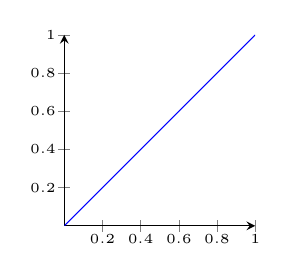
\begin{tikzpicture}
			\begin{axis}[
				membership axes,
			]
				\addplot [blue] {x};
				%{max(gauss(\aOne-2*\bOne*sqrt(-ln(x)), \aTwo, \bTwo), gauss(\aOne+2*\bOne*sqrt(-ln(x)), \aTwo, \bTwo))};
			\end{axis}
		\end{tikzpicture}
		\caption{$\mu_{CP(A,A')}(v)$ при $a_1 = a_2$ и $b_1 = b_2$}
	\end{subfigure}
	\label{fig:ftv-gauss-true}
\end{figure}

На рис. \cref{fig:ftv-gauss-true} представлены графики совпадающих функций принадлежности высказываний и построенной функции принадлежности нечеткого значения истинности.

\item \textit{Аксиома ложности.} Нечеткое значение истинности ЛОЖНО задается нечетким множеством:
\begin{equation*} 
CP(A,A') = \left\{\langle\mu_{CP(A,A')}(v), v\rangle\right\} = \left\{(1-v)/v\right\} = \left\{v/(1-v)\right\}, v \in [0; 1],
\end{equation*}
что выполняется тогда и только тогда, когда утверждаемое высказывание $A$ противоположно утверждаемому в $A'$, т. е. функции принадлежности высказываний $A'$ и $A$ удовлетворяют одному из условий:
\[
	\mu_{A'}(x) = 1 - \mu_{A}(x)
\]
 или
\[
    \mu_{A'}(x) = \left\{
    \begin{alignedat}{2}
        1 - \mu_{A}(x), &\quad x \le x_{max} \\
        0, &\quad x > x_{max}
    \end{alignedat}
    \right.
\]
или
\[
    \mu_{A'}(x) = \left\{
    \begin{alignedat}{2}
        0, &\quad x < x_{max} \\
        1 - \mu_{A}(x), &\quad x \ge x_{max},
    \end{alignedat}
    \right.
\]
где $x_{max} = \textrm{arg\,max}_x \mu_{A}(x)$.

\begin{figure}[ht]
	\newcommand{\aOne}{0.5}
	\newcommand{\bOne}{0.05}
	\newcommand{\aTwo}{0.5}
	\newcommand{\bTwo}{0.05}
	\begin{subfigure}[t]{0.5\textwidth}
		\begin{tikzpicture}
			\begin{axis}[
				membership axes,
				]
				\addplot [black, thick] {gauss(x, \aOne, \bOne)};
				\addlegendentry{$\mu_A(x; a_1, b_1)$};
				\addplot [blue, thick] {1-gauss(x, \aTwo, \bTwo)};
				\addlegendentry{$\mu_{A'}(x; a_2, b_2)$};
			\end{axis}
		\end{tikzpicture}
		\caption{$\mu_{A'}(x; a_2, b_2) = 1 - \mu_A(x; a_1, b_1)$ при $a_1 = a_2, b_1 = b_2$}
	\end{subfigure}
	\begin{subfigure}[t]{0.5\textwidth}
		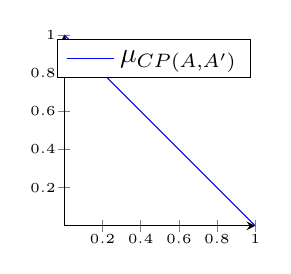
\begin{tikzpicture}
			\begin{axis}[
				membership axes,
				]
				\draw [blue] (0,1) -- (1,0);
				\addlegendimage{blue, no marks, line legend}
				\addlegendentry{$\mu_{CP(A,A')}$}
				%\addplot [blue, thick] {max(gauss(\aOne-\bOne*sqrt(-ln(x)), \aTwo, \bTwo), gauss(\aOne+\bOne*sqrt(-ln(x)), \aTwo, \bTwo))};
			\end{axis}
		\end{tikzpicture}
		\caption{$\mu_{CP(A,A')}(v)$ при $\mu_{A'}(x) = 1 - \mu_A(x)$}
	\end{subfigure}
	\label{fig:ftv-gauss-false}
\end{figure}

На рис. \cref{fig:ftv-gauss-false} представлены графики противоположных по значению функций принадлежности высказываний $A'$ и $A$ и построенной функции принадлежности нечеткого значения истинности.
\item \textit{Аксиома абсолютной истинности.}  Значение истинности АБСОЛЮТНО ИСТИННО задается нечетким множеством:
\begin{equation*}
CP(A, A') = \left\{\langle\mu_{CP(A, A')}(v), v\rangle\right\} = \left\{v/1\right\} = \left\{1/1\right\}, v \in [0, 1],
\end{equation*}
что выполняется тогда и только тогда, когда $A'$ абсолютно соответствует $A$, то есть в случае когда оценка данная в высказываниях $A'$ и $A$ является четкой или нечеткой, когда носитель высказывания $A'$ включен в носитель высказывания $A$.

\begin{figure}[ht]
	\newcommand{\aOne}{0.5}
	\newcommand{\bOne}{0.05}
	\newcommand{\aTwo}{0.5}
	\newcommand{\bTwo}{0.05}
	\begin{subfigure}[t]{0.5\textwidth}
		\begin{tikzpicture}
			\begin{axis}[
				membership axes,
			]
				\addplot [black, thick] {gauss(x, \aOne, \bOne)};
				\addlegendentry{$\mu_A(x)$}
				%\addplot [blue, thick] {gauss(x, \aTwo, \bTwo)};
				\draw [blue, thick] (0,0) -- (\aTwo,0);
				\draw [blue, thick] (\aTwo,0) -- (1,0);
				\draw [blue, thick] (\aTwo,0) -- (\aTwo,1);
				\addlegendimage{blue, thick, no marks, line legend}
				\addlegendentry{$\mu_{A'}(x)$}
			\end{axis}
		\end{tikzpicture}
		\caption{$\mu_A(x; a_1, b_1)$ и $\mu_{A'}(x; a_2, b_2)$ при $a_1 = a_2, b_1 \gg b_2$}
	\end{subfigure}
	\begin{subfigure}[t]{0.5\textwidth}
		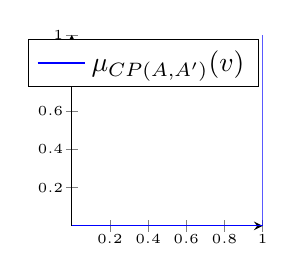
\begin{tikzpicture}
			\begin{axis}[
				membership axes,
			]
				\draw [blue] (0,0) -- (1,0);
				\draw [blue] (1,0) -- (1,1);
				\addlegendimage{blue, thick, no marks, line legend}
				\addlegendentry{$\mu_{CP(A,A')}(v)$}
				%{max(gauss(\aOne-\bOne*sqrt(-ln(x)), \aTwo, \bTwo), gauss(\aOne+\bOne*sqrt(-ln(x)), \aTwo, \bTwo))};
			\end{axis}
		\end{tikzpicture}
		\caption{$\mu_{CP(A,A')}(v)$ при $a_1 = a_2, b_1 \gg b_2$}
	\end{subfigure}
	\label{fig:ftv-gauss-absolute-true}
\end{figure}

На рис. \ref{fig:ftv-gauss-absolute-true} представлены графики функций принадлежности высказывания $A'$, включенного в $A$ и функции принадлежности нечеткого значения истинности, соответствующие данной ситуации. Для моделирования четкого значения функции принадлежности (синглтона) взята гауссова функция кривая с дисперсией, стремящейся к нулю.

\item \textit{Аксиома абсолютной ложности.}  Значение истинности АБСОЛЮТНО ЛОЖНО задается нечетким множеством:
\begin{equation*}
CP(A, A') = \left\{\langle\mu_{CP(A, A')}(v), v\rangle\right\} = \left\{v/0\right\} = \left\{1/0\right\}, v \in [0, 1],
\end{equation*}
что выполняется тогда и только тогда, когда $A'$ абсолютно не соответствует $A$, то есть в случае когда оценки данные в высказываниях $A'$ и $A$ имеют несовпадающие носители.

\begin{figure}[ht]
	\newcommand{\aOne}{0.3}
	\newcommand{\bOne}{0.05}
	\newcommand{\aTwo}{0.67}
	\newcommand{\bTwo}{0.05}
	\begin{subfigure}[t]{0.5\textwidth}
		\begin{tikzpicture}
			\begin{axis}[
				membership axes,
			]
				\addplot [black, thick] {gauss(x, \aOne, \bOne)};
				\addlegendentry{$\mu_A(x)$}
				\addplot [blue, thick] {gauss(x, \aTwo, \bTwo)};
				\addlegendentry{$\mu_{A'}(x)$}
			\end{axis}
		\end{tikzpicture}
		\caption{$\mu_A(x; a_1, b_1)$ и $\mu_{A'}(x; a_2, b_2)$ при $|a_1 - a_2| \gg 0, b_1 \approx b_2$}
	\end{subfigure}
	\begin{subfigure}[t]{0.5\textwidth}
		\begin{tikzpicture}
			\begin{axis}[
				membership axes,
				samples=1000,
			]
				\addplot [blue, thick] {gauss(\aOne+2*\bOne*sqrt(-ln(x)), \aTwo, \bTwo)};
				\addlegendentry{$\mu_{CP(A,A')}(x)$}
			\end{axis}
		\end{tikzpicture}
		\caption{$\mu_{CP(A,A')}(v)$ при $|a_1 - a_2| \gg 0, b_1 \approx b_2$}
	\end{subfigure}
	\label{fig:ftv-gauss-absolute-false}
\end{figure}

На рис. \ref{fig:ftv-gauss-absolute-false} представлены графики непересекающихся гауссовых функций принадлежности высказываний $A'$ и $A$ с удаленными центрами и построенная для этого случая функция принадлежности нечеткого значения истинности.

\item \textit{Аксиома квазиистинности.} Нечеткое значение истинности КВАЗИИСТИННО задается нечетким множеством:
\begin{equation*} 
CP(A,A') = \left\{\langle\mu_{CP(A,A')}(v), v\rangle\right\} = \left\{1/v\right\}, v \in [0; 1],
\end{equation*}
что выполняется тогда и только тогда, когда утверждение в высказывании $A'$ является частным по отношению к $A$, то есть оценка данная в высказывании $A$ интервальная и совпадает с носителем высказывания $A$.

\begin{figure}[ht]
	\newcommand{\aOne}{0.5}
	\newcommand{\bOne}{0.05}
	\newcommand{\aTwo}{0.5}
	\newcommand{\bTwo}{0.05}
	\begin{subfigure}[t]{0.5\textwidth}
		\begin{tikzpicture}
			\begin{axis}[
				membership axes,
				]
				\addplot [black, thick] {gauss(x, \aOne, \bOne)};
				\addlegendentry{$\mu_A(x)$}
				\draw [blue, thick] (0,1) -- (1,1);
				\addlegendimage{blue, thick, no marks, line legend}
				\addlegendentry{$\mu_{A'}(x)$}
			\end{axis}
		\end{tikzpicture}
		\caption{$\mu_A(x; a_1, b_1)$ и $\mu_{A'}(x; a_2, b_2)$ при $a_1 = a_2, b_1 \ll b_2$}
	\end{subfigure}
	\begin{subfigure}[t]{0.5\textwidth}
		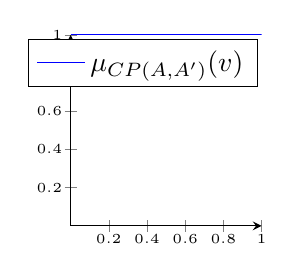
\begin{tikzpicture}
			\begin{axis}[
				membership axes,
				]
				\draw [blue] (0,1) -- (1,1);
				\addlegendimage{blue, no marks, line legend}
				\addlegendentry{$\mu_{CP(A,A')}(v)$}
				%\addplot [blue, thick] {max(gauss(\aOne-\bOne*sqrt(-ln(x)), \aTwo, \bTwo), gauss(\aOne+\bOne*sqrt(-ln(x)), \aTwo, \bTwo))};
			\end{axis}
		\end{tikzpicture}
		\caption{$\mu_{CP(A,A')}(v)$ при $a_1 = a_2, b_1 \ll b_2$}
	\end{subfigure}
	\label{fig:ftv-gauss-quazi-true}
\end{figure}

На рис. \cref{fig:ftv-gauss-quazi-true} представлены графики функций принадлежности нечеткого множества $A$, полностью содержащегося в нечетком множестве $A'$, и рассчитанной функции принадлежности нечеткого значения истинности.

\item \textit{Аксиома квазиложности.} Нечеткое значение истинности КВАЗИЛОЖНО задается нечетким множеством:
\begin{equation*} 
CP(A,A') = \left\{\langle\mu_{CP(A,A')}(v), v\rangle\right\} = \left\{0/v\right\}, v \in [0; 1],
\end{equation*}
что справедливо тогда и только тогда, когда утверждаемое в $A'$ не имеет реального подтверждения в действительности. Иными словами, отсутствует возможность установления истинности высказывания $A'$, так как не определено, существует ли в действительности то, что утверждается в $A'$.

Данную ситуацию нельзя выразить математически и изобразить, поскольку истинность функция принадлежности высказывания $A'$ не может быть оценена.
\end{itemize}

\subsection{Вычисление нечеткого значения истинности, когда функции принадлежности формализуются гауссовыми функциями}

Зададим функции принадлежности нечетких множеств факта и посылки в виде:
\begin{equation*}
\begin{aligned}
\mu_{A}(x; a, b) = e^{-\frac{(x-a)^2}{2b^2}} & \mu_{A'}(x; c, d) = e^{-\frac{(x-c)^2}{2d^2}}. \\
\end{aligned}
\end{equation*}

Тогда, согласно формуле нечеткого значения истинности (\ref{eqn:1-ftv}), для вычисления нечеткого значения истинности в точке $v_0$ необходимо сперва найти все точки из области определения функции принадлежности факта, в которых он принимает значение $v_0$. В случае с гауссовой функцией это можно сделать, с помощью обратной гауссовой функции:
\begin{equation*}
x(v) = a \pm b\sqrt{-2\ln{v}},
\end{equation*}
тогда
\begin{align}
\mu_{CP(A, A')}(v) &= \max\left\{e^{-\frac{((a - b\sqrt{-2\ln v})-c)^2}{2 d^2}},e^{-\frac{((a + b\sqrt{-2\ln v})-c)^2}{2 d^2}}\right\} \nonumber \\
&= \max\left\{e^{-\frac{((a-c) - b\sqrt{-2\ln v})^2}{2 d^2}},e^{-\frac{((a-c) + b\sqrt{-2\ln v})^2}{2 d^2}}\right\} \label{eqn:ftv-gauss-expanded}
\end{align}

%\section{Сравнение нечетких логических систем с нечеткими системами типа Мамдани и Такаги-Сугено}
%
%Нечеткая логическая система использует нечеткую логическую импликацию для связывания антецедента и консеквента в нечетком правиле, а также связку И для агрегации правил.
%
%Нечеткая система типа Мамдани использует t-норму для связывания антецедента и консеквента в нечеком правиле, а также связку ИЛИ для агрегации правил.
%
%Как заключено в [https://ssrn.com/abstract=2900827] 

\section{Применение нечетких моделей для прогнозирования временных рядов}

Для временного ряда $\mathbf{y_t} = (y_1, \dots, y_T)$ величина $y_t$ представляет измеренное значение наблюдаемой переменной в момент времени $t$. Ставится задача предсказания значений $\hat{y}_{t+h}$ для заданного горизонта предсказания $h$.

Модель временного ряда $f(\cdot)$ порядка $p$ использует последние $p$ значений до момента $t$ для оценки значения:
\[
\hat{y}_{t+h} = f(y_{t-p}, \dots, y_t),
\]
где $p$ - размер лагового окна.

При моделировании временных последовательностей с использованием нейро-нечетких систем каждое значение $y_t\in Y$ фаззифицируется в нечеткое множество $A_t$. Эти нечеткие множества составляют множество термов лингвистической переменной $\tilde{A}$, определенной на базовом множестве $Y$. Такая система принимает $p$ входов, а правила в ее базе знаний устанавливают нечеткую последовательно-временную связь в рамках заданного окна $p+1$. Параметр $p$ называется порядком нечеткой системы прогнозирования временных рядов.

База правил в такой системе представляется набором из $N$ правил вида:
\begin{equation}
	\begin{aligned}
		R_k: \textrm{Если }&y_{t-p}\textrm{ есть }A_{k1}\textrm{ и }\dots\textrm{ и } y_{t}\textrm{ есть }A_{kp},&\\
		\textrm{ то }&y_{t+1}\textrm{ есть }A_{k\,p+1},&k\in\overline{1,N},
	\end{aligned}
\end{equation}
где каждое нечеткое отношение $\mathrm{T_1}\left\{A_{k1}, \dots, A_{kp}\right\} \rightarrow A_{k\,p+1}$, заданное в правиле $R_k$, выражает единицу \todo{логических} знаний о моделируемом протекающем во времени процессе.

Входы нечеткой системы по каждому измерению могут описываться одной и той же лингвистической переменной, заданной на базовом множестве области значений временного ряда и имеющей одинаковую порождающую процедуру для терм-множеств.

\subsection{Обучение нечетких систем в контексте задачи прогнозирования временных рядов}

Развитие способов обучения нечетких систем в рамках задачи прогнозирования временных рядов проходило взаимосвязано с адаптацией нечеткого моделирования как непосредственно к задаче регрессии временных рядов, так и к задачам другого рода. Ранние подходы следовали более типовому набору шагов для построения нечетких систем \cite{Chellai2022}. Для формирования набора термов единственно лингвистической переменной $\tilde{A}$ ее пространство значений ограничивалось минимальным и максимальными значениями временного ряда и разбивалось на накладывающиеся друг на друга участки, каждый из которых составлял носитель соответствующего нечеткого множества. В широко цитируемом подходе Чена \cite{Chen1996} разбиение производилось на равные отрезки. Очевидным недостатком такого примитивного способа разбиения пространства значений является несоответствие часто отличному от равномерного распределению функции плотности вероятности этих значений. База правил формировалась напрямую из экземпляров данных, посредством сопоставления каждому экземпляру комбинации термов, имеющих наибольшую степень принадлежности по входам в совокупности, что соответствует довольно популярному из-за своей простоты методу \cite{Wang1992}.

В более поздних методах формирование сразу базы правил с соответствующими терм-множествами из данных, то есть более точное выделение шаблонных отрезков из временных рядов, стало более распространенным подходом, из-за ограничений в увеличении точности нечеткой системы при разбиения базового множества лингвистической переменной $\tilde{A}$ со сложной функцией плотности распределения значений. Таким образом одни и те же методы можно применять для разбиения пространства значений временных рядов (одно измерение) или для разделения пространства окон временных рядов (когда последовательность значений в окне временного ряда интерпретируется как точка в $n$-мерном пространстве). В последнем случае посредством разбиения пространства окон временного ряда может осуществляться формирование базы правил.

Распространенной группой таких методов являются подходы на основе различных алгоритмов кластеризации \cite{Lucas2021}:  \textit{k}-средних, алгоритмы учитывающие плотность распределения точек, агломеративная кластеризация.

Эволюционные подходы, например, Particle Swarm Optimization (PSO)\cite{Davari2009} могут обеспечить оптимальную настройку параметров нечеткой модели при сложной конфигурации обучающего набора данных. Основная сложность использования этих методов состоит в необходимости выполнять большое количество вычислений функции приспособленности на всем обучающем наборе данных на каждой итерации для всех особей популяции. Поэтому для сокращения времени оценки параметров модели стараются минимизировать набор параметров, для которых применяются методы глобальной оптимизации.

Стоит также отметить гибридные подходы построения и обучения нечетких систем моделирования временных рядов в комбинации с другими моделями машинного обучения, такими как, Support Vector Machine (SVM), Long-Sort Term Memory (LSTM), Transformer, и статистические методели, например, Auto Regressive Integrated Moving Average (ARIMA).

Отдельно в случае авторегрессионного прогнозирования временных рядов подходы потокового обучения нечетких систем (\textit{evolving fuzzy systems}, \textit{EFS}). Метод \textbf{participatory learning} --- подход к адаптивному обучению, при котором нечеткая система динамически обновляет свою структуру и параметры, основываясь на степени согласованности новых данных с текущей моделью\cite{Lima2010, Alves2021}.

Описанные выше методы используют для нечеткого вывода методы Мамдани и Такаги-Сугено. Последний особенно популярен в задаче прогнозирования временных рядов.

\subsection{Анализ способов построения нечетких временных моделей}

Для реализации сильных сторон от использования нечеткого моделирования нужно отразить информацию о прогнозируемой величине при выборе метода ее фаззификации. Существующие подходы фаззификации значений временных рядов комбинируют различные формы функций принадлжености, способы оценку истинного значения в термах и формализации неопределенности. В \cite{Pekaslan2020} описан подход к фаззификации измеренных значений временного ряда в нечеткие множества с гауссовыми  функциями принадлежности. Измеренные значения полагаются истинными и задают центры гауссовых функций принадлежности, а среднеквадратичное отклонение оценивается как среднеквадратичная разность между соседними значениями в некотором окне вокруг данной точки во временной последовательности. \todo{Написать формулу} В \cite{Pourabdollah2017} для фаззифицированных таким образом значений в нечеткие множества выполняется переоценка истинных значений посредством преобразования взвешенным скользящим средним центров гауссовой ф. п. нечетких множеств. \todo{Написать формулу} Стоит уточнить, что в этих двух работах рассматривается нечеткий вывод с использованием non-singleton фаззификации.

Для выбора лучшей конфигурации нечеткой модели в задаче регрессии ключевыми метрикам как правило являются \textit{Root Mean Square Error (RMSE)} и \textit{Mean Absolute Error (MAE)}. Выбрать наиболее подходящие методов импликации и дефаззификации также можно изучив эмпирический опыт использования различных вариантов при решении задачи регрессии. В нескольких исследованиях, в которых непосредственно сравнивались операторы импликации в регрессионных задачах, Лукасевич неизменно оказывался лучшим с наименьшим отклонением между прогнозируемыми и фактическими значениями, за ним следовали Райхенбах и Гедель (или Клини–Динес) в большинстве экспериментов \cite{Gkountakou2023}. Напротив, $R$-импликациям, таким как Goguen и Gödel, часто не хватает плавности \cite{Krieken2022}. В \cite{Kiszka1985} операторы, основанные на $S$-нормах (например, Лукасевич, Райхенбах), неизменно давали более низкий RMSE, чем простое минимальное значение (Мамдани), что часто сокращало погрешность на 10-20\% при моделировании параметров двигателя постоянного тока.

Общим практикой является включение метода дефаззификации в набор оптимизируемых гиперпараметров. Для задачи регресии часто используются методы дефаззификации центра тяжести и среднего максимума. Например, в \cite{Ali2022} метод центра тяжести показал лучшее значение метрики RMSE, а в \cite{Yan2010} --- метод среднего максимума.

Также в \cite{Bede2018} была показана лучшая точность прогнозирования временного ряда при использовании импликации Лукасевича и дефаззификации по методу среднего максимума, превзойдя по точности дефаззификацию по методу центра тяжести при импликации Лукасевича и минимуме (Мамдани).

\section{Постановка задачи исследования}

С учетом описанного в разделе \cref{sec:ch1-fuzzy-logical-inference-problem} состояния в области исследования нечеткого логического вывода, а именно: обоснованной примерами прироста качества нечеткого моделирования перехода к использованию несинглтонной фаззификации в моделях типа Мамдани, продемонстрированного несоответствия таких подходов как Мамдани принципам классического нечеткого логическкого вывода, вызванного определенным упрощением, а также низкой проработанностью этих проблем в совокупности в научных публикациях, актуальным является развитие нечеткого логического вывода при несинглтонной фаззификации. Одна из основных задач в этом направлении исследования состоит в преодолении существовавшего до сих пор барьера в виде высокой вычислительной сложности при увеличении количества входов системы.

Изучение возможных решений данной проблемы стоит начать с разбиения нечеткого логического вывода на составляющие математические операции. Описанная выше концепция нечеткого значения истинности предоставляет способ нахождения нечеткой меры сходства входного нечеткого множества и нечеткого множества в антецеденте правила, что по сути соответствует определенной части в композиции операций механизма нечеткого вывода, Кроме того, в литературе определена операция свертки НЗИ для отдельных независимых входов системы в единое пространство, что выносит проблемы обработки нескольких входов системы вывода <<за скобки>> непосредственно нечеткого логического вывода.

Затем нужно выявить особенности и возможные сложности высокопроизводительной реализации выработанного метода при анализе неопределенных данных. Следует организовать вычисления с применением параллельных технологий программирования.

\todo{Поскольку нечеткие системы логического типа демонстрировали хорошую точность в задачах регрессии}

\section{Выводы}

\begin{enumerate}
	\item В ответ на сложность использования канонического нечеткого вывода Заде появился ряд упрощенных методов вывода Мамдани, Такаги-Сугено, Ларсена и Цукамото, тогда как логический подход показывал лучшее качество моделирования в некоторых задачах. Мендель показал как можно использовать фаззификацию типа non-singleton на основе подходов Мамдани и Такаги-Сугено, и продемонстрировал значимый прирост в качестве нечеткого моделирования в некоторых задачах. Вывод основанный на подходах Мамдани, Такаги-Сугено и др. не , в то время как нечеткий вывод логического типа при non-singleton фаззификации остается не исследован.
	\item Нечеткое значение истинности выражает истинность одного нечеткого множества относительно другого в нечетком пространстве истинности. Целесообразно будет выработать механизм эффективного вычисления этой истинности, а затем, рассматривая процедуру нечеткого логического вывода как композицию некоторых операций, внедрить операцию вычисления нечеткого значения истинности в эту композицию. Использование в качестве функции принадлежности нечетких множеств гауссовой функции позволяет легко аналитически выражать операции по вычислению нечеткого значения истинности без потери общности.
	\item Задача прогн
	\item Исходя из обоснования актуальности разработки проблемы нечеткого вывода логического типа и характеристики механизма нечеткого значения истинности , необходимо\dots Выработанный метод нужно адаптировать для высокопроизводительной реализации. Затем полученную реализацию нечеткого логического вывода нужно приметить для решения задачи прогнозирования временных рядов, и оценить качество и производительность реализованной нечеткой логической модели.
\end{enumerate}

\FloatBarrier
